% vim:ts=4:sw=4
%
% Copyright (c) 2008-2009 solvethis
% Copyright (c) 2010-2015 Casper Ti. Vector
% Public domain.
%
% 使用前请先仔细阅读 pkuthss 和 biblatex-caspervector 的文档,
% 特别是其中的 FAQ 部分和用红色强调的部分。
% 两者可在终端/命令提示符中用
%   texdoc pkuthss
%   texdoc biblatex-caspervector
% 调出。

% 采用了自定义的(包括大小写不同于原文件的)字体文件名,
% 并改动 ctex.cfg 等配置文件的用户请自行加入 nofonts 选项;
% 其它用户不用加入 nofonts 选项,加入之后反而会产生错误。
\documentclass[UTF8]{pkuthss}

% 使用 biblatex 排版参考文献,并规定其格式(详见 biblatex-caspervector 的文档)。
% 这里按照英文文献在前,中文文献在后排序(“sorting = ecnty”);
% 若需按照中文文献在前,英文文献在后排序,请设置“sorting = centy”;
% 若需按照引用顺序排序,请设置“sorting = none”。
\usepackage[backend = biber, style = caspervector, utf8, sorting = none]{biblatex}

\graphicspath{{../figure/}}
\DeclareGraphicsExtensions{.eps,.pdf}

% 按学校要求设定参考文献列表中的条目之内及之间的距离。
\setlength{\bibitemsep}{3bp}
% 对于 linespread 值的计算过程有兴趣的同学可以参考 pkuthss.cls。
\renewcommand*{\bibfont}{\zihao{5}\linespread{1.27}\selectfont}

% 设定文档的基本信息。
\pkuthssinfo{
	cthesisname = {硕士研究生学位论文}, ethesisname = {Master Thesis},
	ctitle = {基于FPGA实现的高不可预测性PUF电路设计}, etitle = {Design methodology of Unpredictable PUFs based on FPGA Implementation},
	cauthor = {唐文懿},
	eauthor = {Wenyi Tang},
	studentid = {1301214150},
	date = {2016年四月},
	school = {信息科学技术学院},
	cmajor = {微电子学与固体物理学}, emajor = {Microelectronics},
	direction = {系统集成芯片设计及设计方法学},
	cmentor = {贾嵩}, ementor = {Prof.\ Song Jia},
	ckeywords = {其一,其二}, ekeywords = {First, Second}
}
% 载入参考文献数据库(注意不要省略“.bib”)。
\addbibresource{thesis.bib}

\begin{document}
	% 以下为正文之前的部分,默认不进行章节编号。
	\frontmatter
	% 此后到下一 \pagestyle 命令之前不排版页眉或页脚。
	\pagestyle{empty}
	% 自动生成封面。
	\maketitle

	% 此后到下一 \pagestyle 命令之前正常排版页眉和页脚。
	% 封面要求单面打印,故需新开右页,此处已一并实现。
	\cleardoublepage
	\pagestyle{plain}
	% 重置页码计数器,用大写罗马数字排版此部分页码。
	\setcounter{page}{0}
	\pagenumbering{Roman}

	% 版权声明。
	% vim:ts=4:sw=4
%
% Copyright (c) 2008-2009 solvethis
% Copyright (c) 2010-2015 Casper Ti. Vector
% All rights reserved.
%
% Redistribution and use in source and binary forms, with or without
% modification, are permitted provided that the following conditions are
% met:
%
% * Redistributions of source code must retain the above copyright notice,
%   this list of conditions and the following disclaimer.
% * Redistributions in binary form must reproduce the above copyright
%   notice, this list of conditions and the following disclaimer in the
%   documentation and/or other materials provided with the distribution.
% * Neither the name of Peking University nor the names of its contributors
%   may be used to endorse or promote products derived from this software
%   without specific prior written permission.
%
% THIS SOFTWARE IS PROVIDED BY THE COPYRIGHT HOLDERS AND CONTRIBUTORS "AS
% IS" AND ANY EXPRESS OR IMPLIED WARRANTIES, INCLUDING, BUT NOT LIMITED TO,
% THE IMPLIED WARRANTIES OF MERCHANTABILITY AND FITNESS FOR A PARTICULAR
% PURPOSE ARE DISCLAIMED. IN NO EVENT SHALL THE COPYRIGHT HOLDER OR
% CONTRIBUTORS BE LIABLE FOR ANY DIRECT, INDIRECT, INCIDENTAL, SPECIAL,
% EXEMPLARY, OR CONSEQUENTIAL DAMAGES (INCLUDING, BUT NOT LIMITED TO,
% PROCUREMENT OF SUBSTITUTE GOODS OR SERVICES; LOSS OF USE, DATA, OR
% PROFITS; OR BUSINESS INTERRUPTION) HOWEVER CAUSED AND ON ANY THEORY OF
% LIABILITY, WHETHER IN CONTRACT, STRICT LIABILITY, OR TORT (INCLUDING
% NEGLIGENCE OR OTHERWISE) ARISING IN ANY WAY OUT OF THE USE OF THIS
% SOFTWARE, EVEN IF ADVISED OF THE POSSIBILITY OF SUCH DAMAGE.

\specialchap{版权声明}

任何收存和保管本论文各种版本的单位和个人,
未经本论文作者同意,不得将本论文转借他人,
亦不得随意复制、抄录、拍照或以任何方式传播。
否则一旦引起有碍作者著作权之问题,将可能承担法律责任。

% 若需排版二维码,请将二维码图片重命名为“barcode”,
% 转为合适的图片格式,并放在当前目录下,然后去掉下面 3 行的注释。
%\vfill\noindent
%\includegraphics[height = 5em]{barcode}


	% 中英文摘要。
	% vim:ts=4:sw=4
% Copyright (c) 2014 Casper Ti. Vector
% Public domain.

\begin{cabstract}
信息安全是现在各项系统设计重中之重,单向函数是信息安全协议的基础之一。物理不可克隆函数(PUF)是实现单向函数的一种物理手段,利用未知物理系统的观测点实现激励到响应的映射函数。
PUF适合于有安全性需求的移动端芯片,有着低功耗、高集成度、高安全性等特点。

本文研究了 PUF 在电路系统的实现方法,论文的主要工作和创新点包括:
第一,利用统计方法对现有的多种 PUF 方案进行分析对比,建立数学模型描述电路行为,并从模型特征总结出各 PUF 优劣。
第二,提出了延迟型双稳态 PUF 设计方案,其结合了仲裁型 PUF 和双稳态 PUF 的优点,改进了双稳态 PUF 响应存在偏置的不足,且在 FPGA 上实现了电路并采样验证。
第三,设计了随机脉冲采样 PUF,该结构利用短脉冲传播的不稳定特性,引入随机变量,使得电路行为更加难以建模预测,增强了其抵御建模攻击的能力;同时通过真负边沿采样异或运算,增加了建模的空间复杂度,使得攻击者需要极大量的运算代价对此结构进行建模。最终实验结果显示,设计二具有极好的统计结果和抗建模攻击的能力,其面积开销也是标准 2-XOR PUF 的一半。

最后本文比较了新提出结构在内的多个 PUF 的统计分布、 NIST 测试结果和 SVM 预测结果。
	
\end{cabstract}

\begin{eabstract}
Modern system design concerns more and more about security. As one of the basic foundation of crypto-protocols, one-way function and its implementation takes efforts to do so. Physical Unclonable Functions (PUF) is an alternative to one-way function. PUF ultilizes physical system which is unknown to mankind to set up a projection from challenges to responses. This physical disorder based system, which has low energy consumption and high density, is quite suitable for security portable chips.

In this paper, we analyze and implment PUF in Field Programmable Gate Array, and investigate the randomness, uniqueness and reliability of the PUFs.
We also build models for these PUFs and extract characteristics from the model.
We propose two novel PUF designs. One of them combines the advantage of arbiter PUF and bistable ring PUF, the experiments on FPGA demonstrate it improves the randomness and uniqueness compared to BRPUF.
The other one refered to as random pulse based arbiter PUF, introduces a random bit with a random input pulse signal to confuse the one who wants to model it. The experiment results show the propsoed RPAPUF has a significant increment on space and time complexity of building a model for it.

In the end, we summarize the NIST test results and SVM learning results for all mentioned PUFs.

\end{eabstract}


	% 自动生成目录。
	\tableofcontents

	% 以下为正文部分,默认要进行章节编号。
	\mainmatter
	% 序言。
	% vim:ts=4:sw=4
% Copyright (c) 2014 Casper Ti. Vector
% Public domain.

\specialchap{序言}
信息安全是人类关注的永恒话题。而现代信息安全的大厦是由各种密码协议砌成的,这座大厦的基础就是构筑协议的数学原理。

古典密码学采用的简单映射,如凯撒密码,仿射密码,将原文字符通过线性变换映射成密文字符。由于线性变换的对称性,使得求解逆函数非常容易,这让简单映射密码非常容易受到攻击。最早的非线性加密手段——一次一密密码本——通过不断更换密码表(一种简单哈希表)达到非线性化的目的,只要密码本换的足够勤,那理论上就是不可破解的算法。

现代密码学运用了更深刻的数学知识。以对称加密算法 AES 为例, 128bit AES 加密需要10轮,每一轮都要经过一个非线性运算——S盒——求多项式在$GF(2^n)$上的逆。求逆之后,密钥的每一位都会与明文发生作用,这便使得逆向求解(已知密文、明文求解密钥)非常困难。又来看经典公钥算法 RSA,其用两个大质数分别作为公钥和私钥,利用一种单向函数``大整数的因式分解''使正向运算(求大质数的乘积)简单,而逆向运算(求大整数的因数)非常困难来保证安全性。由此可见,单向函数( One-Way Function )是密码学的基础之一。1945年克劳德·香农( Claude E Shannon )在其经典著作《密码学的数学原理》\supercite{shannon1945mathematical} 指出密码设计的两个原则:扩散( Diffusion )和扰乱( Confusion ),这两个原则也是构造单向函数的原则。扩散指输入变化 1bit 会使输出变化 50\% 的 bits,扰乱指输出的每一个 bit 都是由尽可能多的输出 bit 决定。

在众多的密码系统中,单向函数往往由纯数学概念构造,比如大整数因式分解( RSA )、椭圆曲线求解( ECC )、矩阵分解\supercite{wendt2013bidirectional}( DBF )等等,在实际的电路实现上往往硬件规模较大,或是求值时间较长,在现今有越来越多的便携设备接入网络,而在公共场合下有加密通信的需求,传统的加密方式便不适合应用在这些设备上,所以需要低功耗、低硬件开销的加密方案。

其次,各种便携设备不同于传统主机,流动性大,使得其本身容易被攻击者获取(比如丢失、遭克隆等等手段,而传统攻击者获取的仅仅是信道信息),这使得以物理手段获取旁道信息破译的方法在近几年尤为引人关注。旁道信息是与密文相关的中间信息,呈现方式有很多种,比如加密操作时的功耗、电磁辐射、热辐射、运算错误、存储介质状态等等。利用这些信息,可以快速的破译一些加密系统。如差分功耗分析法,通过相似操作的功耗差值来判断猜解密钥的正确性,大幅度削减了穷举量;又如错误分析,通过手段注入使加密系统产生运算错误,并根据出现错误的时机和现象筛选密钥;而存储介质的分析则通过电磁探测等手段直接观察存储器中的逻辑值,从而提取出关键信息。

针对每一种不同的攻击手段,必须分别采取防御措施。如针对差分功耗分析,使用随机掩码隐藏真正的功耗信息,增加攻击者破解的成本;针对错误注入,加入探测机制阻止系统在出错的时候暴露关键信息;而针对存储介质的攻击,则可以采用 PUF 技术隐式存储关键数据。

在 PUF 技术出现之前,双方通信中关键的密钥往往直接存储在非易失性存储器(如只读存储器 ROM )中。比如门禁系统中门卡的 RFID,只能保存在门卡自身的芯片内。尽管通信协议可以很好的加密通信信道内的数据,但是却不能保护芯片内部 ROM 中的信息。一个恶意攻击者一旦获取了一个门卡,则可以通过技术手段探查 ROM 中的数据提取出关键信息。而 PUF 则以加密系统的物理实现自身特点存储信息,相较于 ROM 等传统非易失性存储器,具有隐秘性好,不可探查等特点,因此受到了相关领域研究者的广泛关注。


Physical Unclonable Function( PUF )最早由 MIT 的理学博士 Pappu S. Ravikanth 于 2001 年提出\supercite{pappu2002physical},而其最初被称为 Physical One-Way Function 。 Ravikanth 在论文中提出了利用可测系统的未知物理状态构造一种 Hash 函数,函数的映射方式由系统的物理特性决定。这种系统必须具有可观测的量以提供输出,同时以人类现有的知识或计算能力不能仿真或计算系统内部的细节,这样攻击者便不会知道系统将提供什么样的输出。 Ravikanth 最后用光学系统实现了他的构想。 PUF 一词则由同是 MIT 的 B. Gassend 等人提出\supercite{gassend2002silicon},值得一提的是, Gassend 将 PUF 的全称写作 Physical Random Function,并称为了不和``伪随机函数''( Pseudo-Random Function )混淆,而写作 Physical Unclonable Function,记作``PUF''。 Gassend 真正提出了基于硅基电路实现的 PUF,他用一系列双口交换器级联的方式,通过检测输出端口延迟先后,将工艺随机波动转换成电平逻辑输出,他的这种电路随后被称为 Arbiter-PUF。不仅如此, Gassend 还提出了一整套 PUF 系统的完善措施,包括输入、输出矫正和 PUF 的实际应用可能,并给出了基于 FPGA 的实验结果,可以说给后来的研究者奠定了完善的基础和研究模板。

自硅基 PUF 提出后, PUF 的研究逐渐演化为几个方向。其一是 PUF 安全性的研究,通过理论和实验提取 PUF 模型参数;其二是 PUF 电路结构的研究,追求更高的可靠性,低功耗和高集成度;其三是 PUF 的应用领域,构建基于 PUF 的密码协议。

2004 年 MIT 的 Daihyun Lim 在其硕士毕业论文\supercite{lim2005extracting}提出对 Arbiter-PUF 建模,并用支持向量机( SVM )拟合出 Arbiter-PUF 的模型参数,开启了机器学习对 PUF 的建模攻击领域。此后,接着机器学习崛起的东风, PUF 研究在攻防两方的博弈中迅速崛起,近几年来吸引了越来越多的研究者和相关会议关注这一领域。

到目前为止, PUF 技术尚未成熟到商用地步,主要有以下几个技术难点。
\begin{itemize}
\item 其一,需要稳定的生成关键数据。系统的物理特征易受环境变化、使用寿命等因素的影响,基于物理特征生成的数据必须克服物理特征波动带来的影响;
\item 其二,安全性。提取的物理特征应不易于被现有技术模拟,不能预测物理特征以破解出关键数据;
\item 其三,实用性。结合上两点,还必须易于实现,以现有技术能在较低成本下制作出来。
\item 最后, PUF 并不适合放在现有的安全系统中,因此有越来越多的文献着手搭建以 PUF 为核心的安全协议,相信随着 PUF 研究的不断深入以及成熟的安全协议的提出, PUF 将会成为安全领域的一颗新星。
\end{itemize}

本文在前人研究基础上,从基本原理入手,分析 PUF 的建模于仿真,针对机器学习建模攻击的应用和防范,主要研究成果有以下几点:
\begin{itemize}
\item 第一,理论分析。对已提出的 PUF 结构进行建模,通过该模型仿真分析其性能指标,成功通过机器学习拟合模型参数;
\item 第二,电路结构。改进 PUF 结构,设计新型的电路结构以达到较高安全性,尤其是对建模攻击的防范;
\item 第三,仿真与实验。在 FPGA 上实现改进电路,通过 PCI-E 接口与 PC 通信,收集并测试大量的输出数据验证其性能指标。
\end{itemize}

文章分为5个章节,此为序章。第\ref{chap:preliminary}章主要阐述本文设计的基础知识;第\ref{chap:buildingmodel}章说明建模方法和安全性理论证明;第\ref{chap:dbrpuf}、\ref{chap:rpapuf}章则阐述本文提出的两种改进结构以及在 FPGA 的实现方法和实验结果;最后第\ref{chap:conclusion}章进行总结和提出展望。

	% 各章节。
	% vim:ts=4:sw=4
% Copyright (c) 2014 Casper Ti. Vector
% Public domain.

\chapter{预备知识}\label{chap:preliminary}
% 中文测试文字。
本章将文中所需要涉及的必要知识进行梳理和阐述,相关概念的定义和简介,不涉及具体证明过程。

\section{PUF工作原理}%
\subsection{工艺涨落}%
集成电路芯片制作可分为设计——流片——验证三大环节。
其中设计者输出给流片厂商的是版图信息。版图则对应着制程中每一层掩膜版的图形,具体到晶体管设计上,版图包括了晶体管宽长比,掺杂区域,互联方式等信息,结合工艺常数,决定了晶体管的设计属性。
在实际流片中,图形转移过程存在套刻精度、刻蚀精度,以及掺杂过程中的退火控制精度等问题。这些操作在实际中存在不可避免的随机误差和系统误差。系统误差在晶圆片上表现为 TT, FF, SS, SF 等不同片区,而随机误差则使得每一颗芯片的时序特征不同,也就是每一个晶体管的表征阈值电压均不相同。
从根本上来说,由于测量系统的局限性,永远不可能复制原子的所有信息,也即不可能使制作后晶体管数值与设计值完全相同。故而误差的累积则造成了工艺涨落,即流片后的晶体管属性与设计属性存在偏差,且在统计学上偏差满足一定的分布规律,下一节将详细说明如何利用由工艺涨落带来的不匹配。
\subsection{信息转换}
由于无法控制工艺涨落的具体数值,也无法预测涨落的大小,因此``芯片制作''这个物理过程符合PUF所要求的``可测不可知''的物理系统,接下来阐述如何给出工艺涨落的观测点。

\begin{figure}[htb!]
\centering
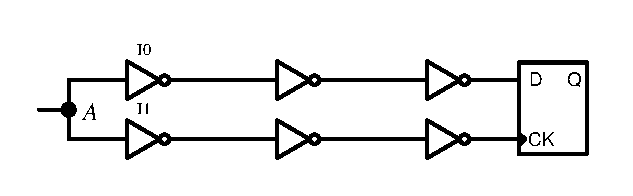
\includegraphics[width=.8\linewidth]{delay-puf}
\caption{延迟-仲裁型 PUF}
\label{fig:delay-puf}
\end{figure}
 
 \begin{figure}[htb!]
 \centering
 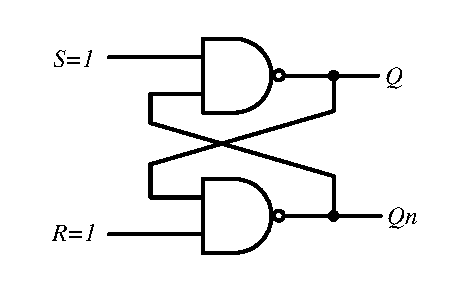
\includegraphics[width=.5\linewidth]{latch-puf}
 \caption{锁存式 PUF}
 \label{fig:latch-puf}
 \end{figure}

PUF将电路工艺参数涨落转换为可输出的电压或电流信号。如图\ref{fig:delay-puf}所示,其中每个反相器和相邻反相器之间的布线在设计上是全等的,但工艺涨落使得反相器中晶体管导电能力必有差异,那么反相器 $ I_0 $ 的信号延迟 $ \Delta t_0 $ 和 $ I_1 $ 的信号延迟 $ \Delta t_1 $ 定满足关系 $ \Delta t_0-\Delta t_1\neq 0 $ ,当输入一个上升沿信号 $ u(t) $ 后, A-D, A-CK  的延迟分别是 $ T_0,T_1 $ ,仲裁器负责判断 D 节点和 CK 节点信号跳变的先后,一个典型的D触发器即可满足仲裁功能。若 D 点信号先于 CK 点上跳,则仲裁器输出逻辑``1'',反之则输出逻辑``0''。由于在得到输出之前并不知道每个反相器的实际延迟,所以不能预测仲裁器的输出,而且每一块相同设计芯片之间的输出也因涨落分布的不同而有差异,因此这样的电路逻辑完成了从工艺涨落到电平信号的信息转换。

又如图\ref{fig:latch-puf}所示,两个反相器及布线在设计上是全等的,上电初始电路处于亚稳态,由于实际的反相器存在偏差,导致其中一个节点的充电电流稍大于另一个节点,使得电路大概率由亚稳态向其中一个稳态过度,此大概率得到的稳态也是工艺涨落的体现,这样的电路也完成了从工艺涨落到存储逻辑值的信息转换。值得注意的是,这里使用了``大概率''的说法,是因为在由亚稳态到稳态的弛豫时间中,存在噪声干扰,从而导致电路向工艺无关的方向变化,这是 PUF 设计中不愿看到的事情。有关 PUF 稳定性的问题,参见\ref{subsec:metrics}节。

\subsection{Weak PUF和Strong PUF}\label{subsec:weakpuf}
类似于\ref{fig:delay-puf}和图\ref{fig:latch-puf}中的电路,利用物理过程的不可控和不可预测性,表达一位或多位稳定信号的系统被称为物理不可克隆函数( Physically Unclonable Function ),其不一定局限于硅基电路,事实上, PUF 概念的首次提出是在光学系统上实现的\supercite{pappu2002physical}。

如果将图\ref{fig:latch-puf}中的结构排成阵列,加上行列选择和译码电路,则构成了类似 SRAM 的阵列,通过不同的``地址''信号可以输出不同的单元信息,像这样的``地址信号''在 PUF 中被称为激励( Challenge ),输出信号被称为响应( Response )。每一个响应都由一个激励相对应,将它们合称为激励-响应对( C-R Pair, CRP )。

\textbf{定义:}若一个 PUF 的激励响应对很少,则称其为 Weak PUF;反之,激励响应对数量级非常多的则称为 Strong PUF\supercite{ruhrmair2014pufs}。

Weak PUF CRP比较单一,没有对外的 IO 接口,以防被穷举,直接将生成的信号送入后续逻辑,实现方式有 SRAM PUF, SA PUF, Latch PUF 等等\supercite{schrijen2012comparative,koeberl2012practical,xiao2014bit,maes2014countering,bhargava2013high}, Weak PUF 多应用于随机数生成、密钥存储方面;

Strong PUF CRP空间非常大,存在对外的 IO 接口,允许通过输入不同的激励得到一组响应,而 CRP 集合的元素量级决定了不可能穷举完所有的 CRP。实现方式有 Arbiter PUF, RO PUF 等等,可实现多种协议。

可以看出 Weak PUF 和 Strong PUF 只是人为地划分,没有明确界限,相较而言,目前以 Strong PUF 的研究和应用居多\supercite{rostami2014quo}。

\subsection{评价指标}\label{subsec:metrics}
PUF (这里特指 Strong PUF,后同)可以用以下几个特定指标衡量:
\begin{itemize}
\item 随机性——对任何一个 CRP 集合的子集,响应(简称 R,后略)的分布应尽可能满足平均分布;
\item 独特性——对任何一个特定的激励(简称 C,后略),一组 PUF 的响应的分布应尽可能满足平均分布;
\item 可靠性——对同样的激励在不同环境温度、电源电压下重复操作应给出相同或大概率相同的响应;
\item 安全性——应对各种已知攻击,详见下一节。
\end{itemize}

除此之外,还有电路通用的面积、功耗、速度等指标,也有用NIST,熵等统计工具代替上述公式\supercite{van2013bias,koeberl2014entropy},特定指标优先级高于通用指标。

下面给出1-3指标的数学定义:

设激励 C 集合$ {c_i} $,响应 R 集合$ {r_i} $,$ r_i=f(c_i) $,若$ R={0,1} $,则随机性可以表征为:
\begin{equation}\label{eq:metric-rand}
Rand=\frac{1}{N}\cdot\sum^{N}f(c_i)
\end{equation}
$ N $ 为 CRP 测试集元素总数,随机性期望值为$ 0.5 $,表明响应应在随机选取的激励下呈平均分布;

独特性表征为:
\begin{equation}\label{eq:metric-uniq}
Uniq=\dfrac{2}{M(M-1)}\sum_{i=1}^{M}\sum_{j=i+1}^{M}\frac{HD(P_i,P_j)}{N}
\end{equation}
\begin{equation}\label{eq:metric-uniq2}
P_i=<f_i(c_0),f_i(c_1),...,f_i(c_n)>
\end{equation}
其中 $ M $ 为测试 PUF 设备总数, $ N $ 为测试激励总数, $ P_i $ 为第 i 个设备 N 个激励响应组成的向量, $ HD(P_i,P_j) $ 指 $ P_i,P_j $ 之间的汉明距离。
独特性期望值为$ 0.5 $,表明任意激励的响应在不同设备间应呈平均分布;

可靠性表征为:
\begin{equation}\label{eq:reliability}
Reliability=\dfrac{1}{MN}\sum_{j}^{M}\sum_{i}^{N}|f(c')-f^{(j)}(c_i)|
\end{equation}
其中N为测试激励总数, $ M $ 为测试重复次数, $ c’ $ 为参考激励,保持不变。可靠性期望值为0。


\section{PUF安全性问题}\label{sec:puf_security}

\subsection{物理模型}
虽然不能精确模拟流片时的掺杂、退火等行为,但是还是可以从宏观上表征一个 PUF 的行为,成这种方式为建模。通常可以将门级电路的驱动能力、延时等抽象为一个平均值W,将R视为C和W的映射 $ R=f(C,W) $。同时,一个好的物理模型有助于快速且准确的仿真验证。

\subsection{参数拟合}
由于 Strong PUF 开放IO端口的特点,若根据攻击者已掌握的一组 CRP 子集,根据建模特点,用机器学习算法拟合出抽象参数$ W $,便可将$ C,W $带入模型中得到 CRP 全集,根据预测率的高低可确定模型建立是否准确抽象了 PUF 的特点。严格来讲,如果一类 PUF 可以被准确抽象出模型,则称该 PUF 是不安全的。但考虑到不是所有模型都能在有限时间内拟合出参数,所以一般认为在特定场合可接受的时间内不能被拟合出参数的 PUF 是安全的。

\section{机器学习算法简介}

\subsection{支持向量机}
支持向量机(Support Vector Machine,SVM),是一种经典的模式识别算法,是 Bell 实验室的 Corinna Cortes 和 Vladimir Vapnik 于1995年首先提出的算法,后经改进,广泛应用于非线性函数拟合,模式识别等机器学习应用中\supercite{cortes1995support}。

SVM 的基本思想是将输入数据映射到一个n维空间中,找到n维空间中的一个超平面能将测试数据集划分开,则该平面将整个空间划分为二,对应着两类不同的数据(如图所示)。

\begin{figure}[h]
\centering
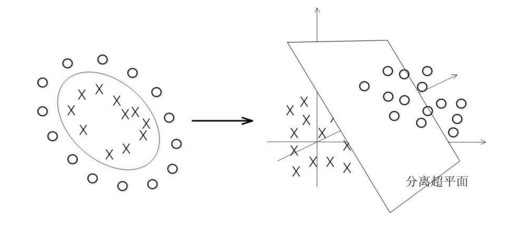
\includegraphics[width=\linewidth]{svm_teach.jpg}
\caption{SVM 映射示意图}
\label{fig:svm_proj}
\end{figure}

下面我们给出线性 SVM 的描述。考虑在n维空间中存在m个特征向量 $ x_1,x_2,x_3,…,x_m $,每个向量具有一个标签( label )``0''或者``1'',期望找到一个超平面( Hyperplane )
\begin{equation}
g(x)=w'x+b=0
\end{equation}
其中 $ w $ 和 $ b $ 是超平面的系数向量。$ g(x) $可以将特征向量分为两类,使得标签``1''向量都满足 $ g(x_i )>0 $,而标签``0''向量都满足 $ g(x_i )<0 $。定义:
\begin{equation}
\gamma=\frac{g(x)}{||w||}
\end{equation}
为向量x到超平面$ g(x)=0 $的几何距离,其中
$ ||w||=\sqrt{w_1^2+w_2^2+...+w_n^2} $
是系数向量w的范数。
为了增加分类的可信度,我们需要找到一个超平面,使得所有特征向量到该超平面的几何距离最大。

事实上并不是所有的数据都是线性可分的,即不存在一个超平面可以将数据集按标签分开。因此非线性 SVM 的做法通常是:
将数据由n维空间映射到$ n+k $维,使得在$ n+k $为空间中数据线性可分。

\subsection{SVM与PUF建模攻击}
如果 PUF 的模型是 $ r=f(c)=sgn(\omega'c+b) $ 的形式,其中 r 是响应,c 是激励,$ \omega $ 是 PUF 内在属性,$ sgn() $是一个符号函数。可以看出 $ g(c)=\omega'c+b=0 $ 便类似于 SVM 中的超平面,在 c 所在空间中,$ g(c) $将向量 c 按标签 r 分为了两类。通过 SVM 找到使 $ \gamma=\frac{g(c)}{||\omega||} $最大的$ \omega $,以使模型达到最大可信度。 SVM 的求解过程在 Matlab 中以 SMO 算法封装实现,而且求解过程并不是本文的关注点,所以不在这里赘述。


\section{相关工作}\label{sec:relatedwork}
\subsection{仲裁型PUF}\label{subsec:apufmodel}
图\ref{fig:delay-puf}展示了一个简单的仲裁型 PUF,图\ref{fig:arb-puf}是一个完整的仲裁型 PUF。其中激励 $ c_i $ 控制双口交换器使得:
\begin{eqnarray}
O_0=c_i?I_1:I_0\\
O_1=c_i?I_0:I_1
\end{eqnarray}
$ O_0,O_1 $ 是交换器的输出, $ I_0,I_1 $ 是输入。这样不同的激励选定了不同的两条数据通路做延迟对比,使得 CRP 空间有 $ 2^n $ 个元素,n为级数。

\begin{figure}[htb!]
\centering
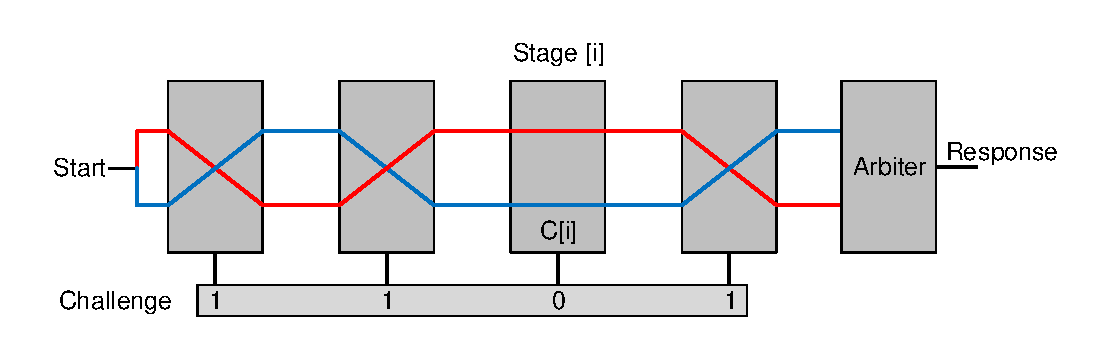
\includegraphics[width=\linewidth]{arbiter_puf}
\caption{仲裁型PUF}
\label{fig:arb-puf}
\end{figure}

将每一个交换器抽象为4条通路,设每条通路延迟分别为 $ p_i,q_i,r_i,s_i $ (如图\ref{fig: switcher}所示),信号到达输入的时间分别为 $ t_1(i),t_2(i) $,输出的时间分别为 $ t_1(i+1),t_2(i+1) $,则有:
\begin{eqnarray}\label{eq:apuf-cell}
t_1(i+1)=c_i?t_2(i)+r_i:t_1(i)+p_i \\
t_2(i+1)=c_i?t_1(i)+q_i:t_2(i)+s_i
\end{eqnarray}

\begin{figure}[htb!]
\centering
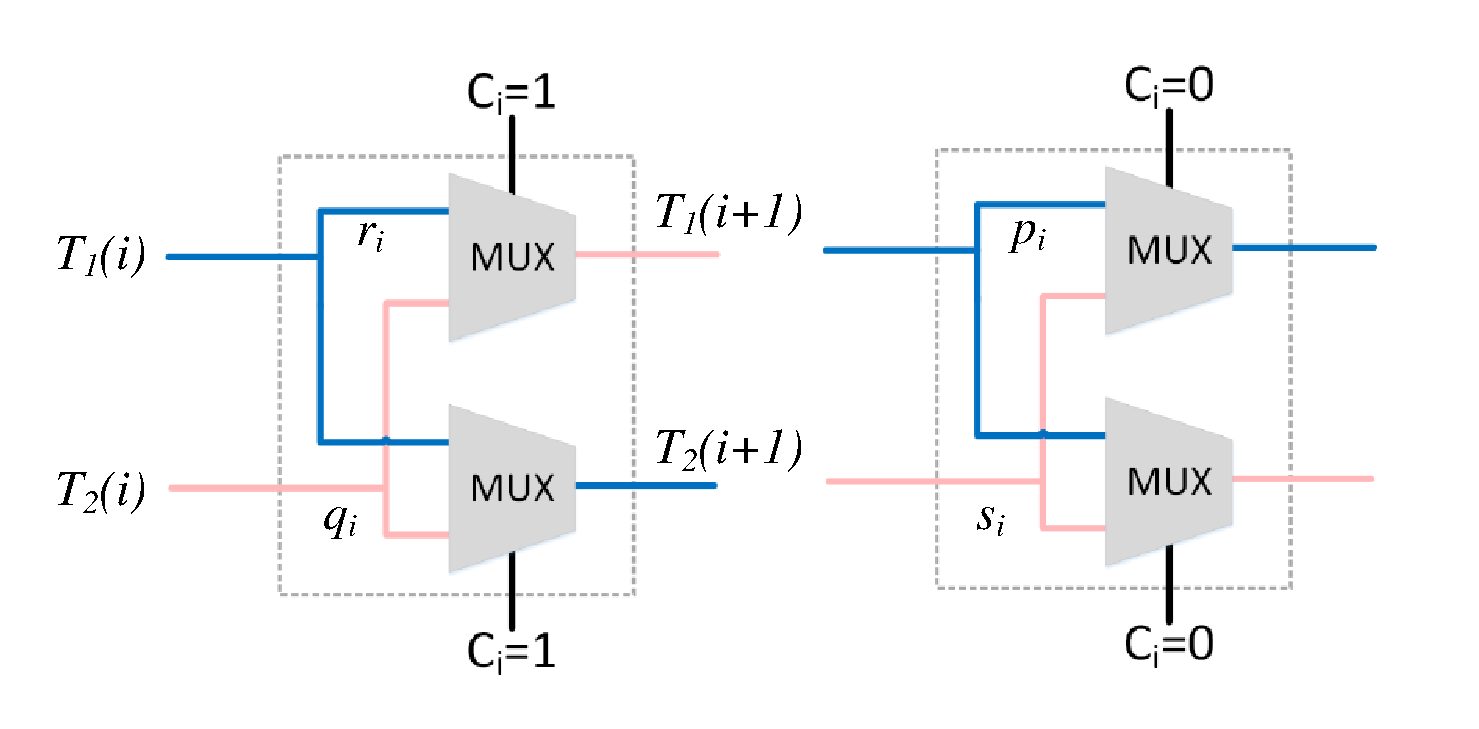
\includegraphics[width=\linewidth]{switcher}
\caption{双口交换器模型}
\label{fig: switcher}
\end{figure}

为了方便数学推导,将逻辑``0''记为-1,将逻辑``1''记为+1,则``异或''等价``乘''运算,故\ref{eq:apuf-cell}可化为
\begin{eqnarray}
t_1(i+1)=\frac{1+c_i}{2}(t_2(i)+r_i)+\frac{1-c_i}{2}(t_1(i)+p_i) \\
t_2(i+1)=\frac{1+c_i}{2}(t_1(i)+q_i)+\frac{1-c_i}{2}(t_2(i)+s_i)
\end{eqnarray}
两式做差得:
\begin{equation}
\delta (i+1)=t_1(i+1)-t_2(i+1)=-c_i\delta(i)+\frac{r_i-q_i+p_i-s_i}{2}+\frac{c_1}{2}(r_i-q_i-p_i+s_i)
\end{equation}
求解此递推关系式最终可得:
\begin{equation}
\delta(n)=p'd
\end{equation}
其中向量 $ p=<p_0,p_1,…,p_n> $, $ p_i=\Pi_{k=i+1}^{n}c_k $,向量 $ d=<\alpha_1,\alpha_2+\beta_1,…,\alpha_n+\beta_(n-1),\beta_n> $, $ \alpha_i=\frac{r_i-q_i-p_i+s_i}{2},\beta_i=\frac{r_i-q_i+p_i-s_i}{2} $,并定义 $ p_n $ 为常数1。由于 $ r=f(c)=sgn[\delta(n)] $,所以存在n维空间上的超平面 $ p'd=0 $ 将特征向量p按r标签分开。在这里p是向量c在同维空间中的一个映射,而向量d代表了每个交换器的延迟时间,是 PUF 的本征属性。

通过一组已知的 CRP 子集,我们可以确定一组向量d,用 SVM 算法找到具有最大可信度的d向量,作为延迟时间的估值,这样便推导出了仲裁型 PUF 的模型,对于未知响应的激励 $ c’ $,根据 $ sgn(p'd) $ 可预测其响应。根据文献\parencite{lim2005extracting}的数据,当训练集大小超过2000时,预测准确率在95\%以上。

\subsection{仲裁型PUF的改进}
因为仲裁型 PUF 的观测点——延迟时间的累加是线性过程,所以容易建立适合 SVM 算法的模型。在文献\parencite{lim2005extracting}中作者提出了改进方案——前馈仲裁型 PUF (如图\ref{fig: ffpuf}),用中间值 $ sgn[\delta(k)] $ 作为交换器的控制信号,如果用同样的思路建立模型,那么在模型表达式中存在非线性函数$ sgn $,不能再直接使用 SVM 算法求解代表延迟的d向量。

\begin{figure}[htb!]
\centering
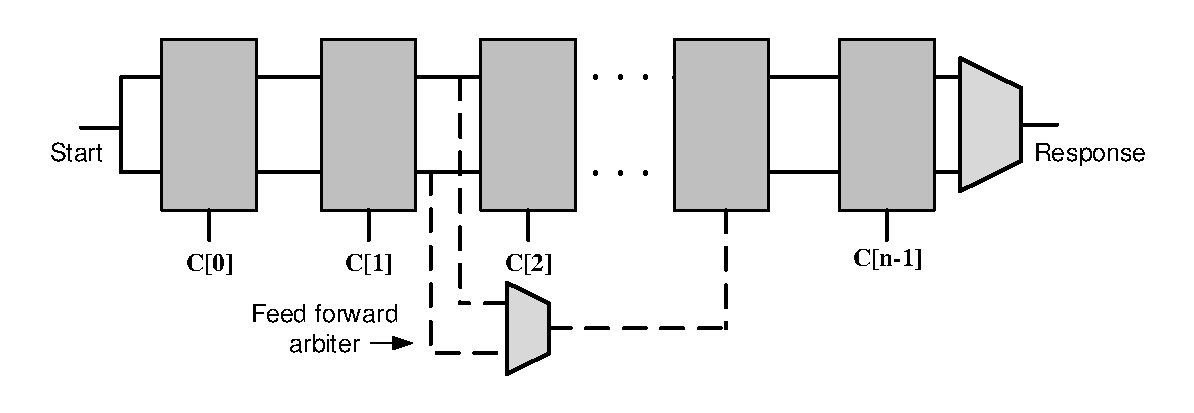
\includegraphics[width=\linewidth]{feedforwardpuf}
\caption{前馈仲裁型 PUF}
\label{fig: ffpuf}
\end{figure}

但\parencite{lim2005extracting}中同样提到了 FFPUF 的攻击方法,而且可以在有限时间内完成,说明这种方法或单独使用这种方法仍是不安全的。

\subsection{异或输出的PUF}\label{subsec:xormethod}

\parencite{suh2007physical}中, G. Edward Suh 和 S. Devadas 提出了 XOR PUF,即是将采用多个传统仲裁型 PUF,给予相同的激励,并且将响应值全部异或起来。异或运算具有非线性特性,具体来讲,两个同激励的 PUF 异或之后输出可以表达成:
\begin{equation}\label{eq:xor-model}
R=p'd\times p'e
\end{equation}
d, e 分别代表两个 PUF 的内在参数,若要使R线性可分,必须要写成 $ P’D $ 的形式,将式\ref{eq:xor-model}展开可以写成 $ P’D $ 的形式,但在这里$ D $是 $ \frac{n(n-1)}{2} $ 维的向量, SVM 的计算复杂度由n上升到了 $ n^2 $,经过多个 PUF 异或后可以将运算复杂度上升到不能在有限时间尺度上求解。

异或的非线性特性不依赖于具体的 PUF 形式,因此是一种通用的增加 PUF 安全性的做法。但是异或的缺点显而易见:面积资源开销增加了N倍,同时误码率也增加了。

\subsection{双稳态环路PUF}
2011年Qingqing Chen等人在会议 Hardware-Oriented Security Transaction 上提出了一种新的PUF,双稳态环路型 PUF(Bistable Ring PUF,如图\ref{fig: brpuf})。  BRPUF 采用了偶数级反相器级联构成回路具有双稳态的特性构建 PUF 的观测点,具有新颖性,并且作者声称其环路具有非线性结构,较传统仲裁型 PUF 安全性更高\supercite{chen2011bistable}。

截止本文撰写时,仅有 Qingqing Chen 本人在文献\parencite{chen2012characterization}中对 BRPUF 做了特性分析; D. Schuster 和 R. Hesselbarth 对 BRPUF 用单层神经网络进行建模\supercite{schuster2014evaluation}。

\begin{figure}[htb!]
\centering
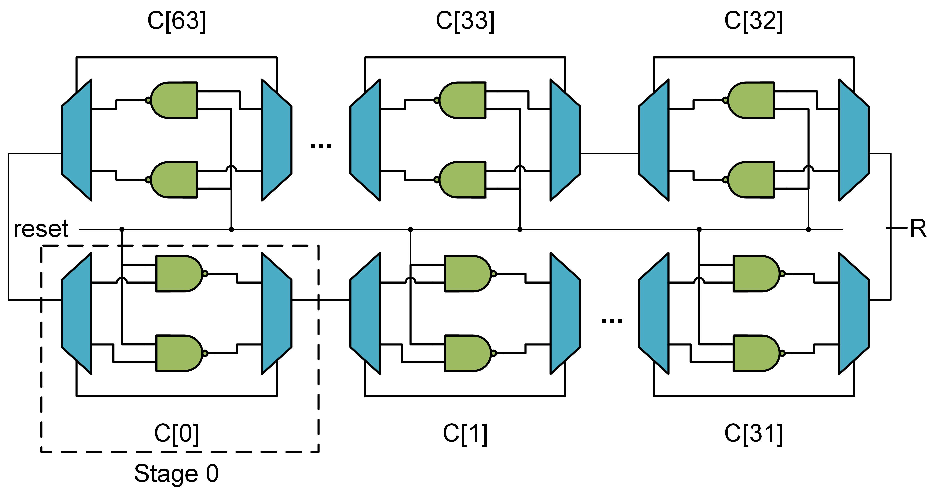
\includegraphics[width=\linewidth]{BRPUF}
\caption{双稳态环路型PUF}
\label{fig: brpuf}
\end{figure}

\section{本章小结}
本章介绍了 PUF 工作机制, PUF 的评价标准;介绍了针对 PUF 的机器学习建模攻击算法;以及列举了近期相关研究者的工作。 PUF 适合生成片间无关的大量激励-响应数据对,且占用资源和功耗相较于传统电路非常小,适合于物联网移动端芯片的内嵌安全模块。
但是目前 PUF 面临建模攻击的威胁,强大的机器学习算法可以用很小的代价推算出 PUF 的所有信息,这样致使一般的 PUF 原型设计不能直接应用于工程芯片。大量的研究者给出了新的设计方案,在下一章中,本文将对其中一个设计进行分析,并提出 PUF 设计的指导性标准。

	% 结论。
	% vim:ts=4:sw=4
% Copyright (c) 2014 Casper Ti. Vector
% Public domain.

\specialchap{结论}\label{chap:conclusion}
\section{全文总结}
在密码学研究中,单向函数是构造高层次密码协议的基础。 PUF 作为物理不可克隆函数,是基于人类不可知的物理原理构造的单向函数,在密码学领域有着重要应用。

本文从数学原理出发,用统计方法和机器学习建模攻击对仲裁型 PUF、异或 PUF、双稳态环路 PUF 进行分析。
通过模型公式对 Strong PUF 的安全性原理进行了总结,分析并指出了异或结构的安全性原理,和双稳态环路 PUF 的统计性失准的原因:因为 BRPUF 在求值过程中累积了所有逻辑门的延迟偏差,导致结果的统计方差大大增加。
根据建模分析,在模型线性表达式或近似线性表达式中,最小线性可分维度的大小决定了机器学习的拟合时间代价。

为了提升 PUF 的安全性,本文提出了两种新型 PUF 结构,其中第\ref{chap:dbrpuf}章的 DBRPUF 针对 BRPUF 进行改进,消除了延迟偏差累积,因此改善了统计测试结果,但相比传统异或结构仍显不足;
第\ref{chap:rpapuf}章新提出的随机脉冲信号的 RPAPUF,利用逻辑门的双边延迟构造出复杂的结构,随机选择脉冲输入,利用脉冲传递路程长短``欺骗''攻击者,使其不能分辨出哪些响应符合模型计算结果,哪些是随机项,从而使建立模型需要花费极大开销,相对传统结构大大加强了 PUF 对于建模攻击的抵御能力。

在实验上,为了缩短仿真时间,本文利用 HSPICE 和 Matlab 结合的方法,HSPICE 负责仿真基本逻辑门的工艺波动,Matlab 负责建立由多个逻辑门组成的电路结构,并通过简化模型静态仿真电路行为,使得多比特 PUF 可以在有限时间内仿真完成。
因此本文验证了所有 PUF 结构,并在 Altera FPGA 上实现并比较了 Arbiter PUF,BRPUF 和 DBRPUF 结构。结果证实了理论分析,证明了本文提出结构的可行性。

最后,本文研究仍存在一些不足之处。
首先,本文采用的统计分析基于工艺波动服从正态分布这一假设,但是在不同工艺,尤其是深亚微米制程下,这一假设不一定满足,因此不同工艺对于 PUF 的输出影响需要进一步的实验验证。
其次,FPGA 的实现存在布线偏差,且实验用 FPGA 数量不足,不能很好的反应不同 PUF 之间的片间分布差异,因此更精确的验证应该采用全定制方法设计 PUF。
最后,本文尚没有对 PUF 的稳定性进行验证,包括电压波动稳定性、环境温度波动稳定性、和时间稳定性。

我们希望在后续的研究中将提出的 RPAPUF 应用于高层次密码协议,从而分析 PUF 的实用性开销和代价,并通过流片进一步验证新型 PUF 结构在不同工艺下的表现,以及在不同电源电压和环境温度下稳定性表现。


\section{前景展望}

PUF 的安全性始终是 PUF 的终极评价标准,而 PUF 的安全性设计和针对这项设计的攻击一直以来都是彼此的博弈。
目前,侵入式探查、旁道攻击等崭新方式给 PUF 带来更多的设计挑战,而全新的工艺技术和期间技术又给 PUF 设计带来了新的可能\supercite{delvaux2013side,merli2013localized,helfmeier2013cloning}。
不仅有双值逻辑的数字电路 PUF,还有基于 RRAM、模拟电路实现的 PUF 具有更高的非线性特点\supercite{liu2015experimental,chen2015utilizing}。
这些都使得未来的研究非常有趣,无论攻防哪一方占得先机,都会给这一领域的研究带来新的启迪和方向。

再者,安全应用的最终实现还是种种密码协议。
基于 PUF 的密码协议越来越多的涌现出来,比如有基础协议``不经意传输协议''的 PUF 实现\supercite{ruhrmair2010oblivious}, FPGA 上的 IP 保护\supercite{kumar2008butterfly}, ``比特承诺协议''\supercite{ruhrmair2013practical}等等。
尽管 PUF 有着天然的安全属性,但是协议的复杂性使基于 PUF 的协议构建非常困难,尤其是每一篇新的协议模型总会伴随而来一篇攻击方法\supercite{ruhrmair2013pufs}。
在未来,相信随着 PUF 研究的深入,能够找到一种完美利用 PUF 特点,真正实现高效、低功耗、不可克隆的密码协议,使得 PUF 应用于千千万万移动端安全芯片,真正为千家万户的安全护航。

	% 正文中的附录部分。
	\appendix
	% 排版参考文献列表。
	\printbibliography[
		% 使“参考文献”出现在目录中;如果同时要使参考文献列表参与章节编号,
		% 可将“bibintoc”改为“bibnumbered”。
		heading = bibintoc,
		% 单独设定排序方案。此设定会局部覆盖之前的全局设置。
		% 注:只有同时使用 2.x 或之后版本的 biblatex 和相应兼容版本的 biber,
		% 才能对每个 \printbibliography 命令采用不同的排序方案,
		% 否则只能在载入 biblatex 宏包时就(全局)指定排序方案。
		% 在这样的情况下,请去掉所有的 sorting 选项,否则可能出错。
		% 此外,biblatex 3.0 中 \printbibliography 的 sorting 选项失效,
		% 详见 biblatex-caspervector 的文档。
		sorting = ecnty
	]
	% 各附录。
	% vim:ts=4:sw=4
% Copyright (c) 2014 Casper Ti. Vector
% Public domain.

\chapter{附件}
% 中文测试文字。




	% 以下为正文之后的部分,默认不进行章节编号。
	\backmatter
	% 致谢。
	% vim:ts=4:sw=4
% Copyright (c) 2014 Casper Ti. Vector
% Public domain.

\chapter{致谢}
% 中文测试文字。



	% 原创性声明和使用授权说明。
	% vim:ts=4:sw=4
%
% Copyright (c) 2008-2009 solvethis
% Copyright (c) 2010-2015 Casper Ti. Vector
% All rights reserved.
%
% Redistribution and use in source and binary forms, with or without
% modification, are permitted provided that the following conditions are
% met:
%
% * Redistributions of source code must retain the above copyright notice,
%   this list of conditions and the following disclaimer.
% * Redistributions in binary form must reproduce the above copyright
%   notice, this list of conditions and the following disclaimer in the
%   documentation and/or other materials provided with the distribution.
% * Neither the name of Peking University nor the names of its contributors
%   may be used to endorse or promote products derived from this software
%   without specific prior written permission.
%
% THIS SOFTWARE IS PROVIDED BY THE COPYRIGHT HOLDERS AND CONTRIBUTORS "AS
% IS" AND ANY EXPRESS OR IMPLIED WARRANTIES, INCLUDING, BUT NOT LIMITED TO,
% THE IMPLIED WARRANTIES OF MERCHANTABILITY AND FITNESS FOR A PARTICULAR
% PURPOSE ARE DISCLAIMED. IN NO EVENT SHALL THE COPYRIGHT HOLDER OR
% CONTRIBUTORS BE LIABLE FOR ANY DIRECT, INDIRECT, INCIDENTAL, SPECIAL,
% EXEMPLARY, OR CONSEQUENTIAL DAMAGES (INCLUDING, BUT NOT LIMITED TO,
% PROCUREMENT OF SUBSTITUTE GOODS OR SERVICES; LOSS OF USE, DATA, OR
% PROFITS; OR BUSINESS INTERRUPTION) HOWEVER CAUSED AND ON ANY THEORY OF
% LIABILITY, WHETHER IN CONTRACT, STRICT LIABILITY, OR TORT (INCLUDING
% NEGLIGENCE OR OTHERWISE) ARISING IN ANY WAY OUT OF THE USE OF THIS
% SOFTWARE, EVEN IF ADVISED OF THE POSSIBILITY OF SUCH DAMAGE.

{
	\CTEXsetup[
		format+ = {\centering}, beforeskip = {40bp}, afterskip = {15bp}
	]{section}

	\specialchap{北京大学学位论文原创性声明和使用授权说明}
	\mbox{}\vspace*{-3em}
	\section*{原创性声明}

	本人郑重声明:
	所呈交的学位论文,是本人在导师的指导下,独立进行研究工作所取得的成果。
	除文中已经注明引用的内容外,
	本论文不含任何其他个人或集体已经发表或撰写过的作品或成果。
	对本文的研究做出重要贡献的个人和集体,均已在文中以明确方式标明。
	本声明的法律结果由本人承担。
	\vskip 1em
	\rightline{%
		论文作者签名:\hspace{5em}%
		日期:\hspace{2em}年\hspace{2em}月\hspace{2em}日%
	}

	\section*{%
		学位论文使用授权说明\\[-0.33em]
		\textmd{\zihao{5}(必须装订在提交学校图书馆的印刷本)}%
	}

	本人完全了解北京大学关于收集、保存、使用学位论文的规定,即:
	\begin{itemize}
		\item 按照学校要求提交学位论文的印刷本和电子版本;
		\item 学校有权保存学位论文的印刷本和电子版,
			并提供目录检索与阅览服务,在校园网上提供服务;
		\item 学校可以采用影印、缩印、数字化或其它复制手段保存论文;
		\item 因某种特殊原因需要延迟发布学位论文电子版,
			授权学校在 $\Box$\nobreakspace{}一年 /
			$\Box$\nobreakspace{}两年 /
			$\Box$\nobreakspace{}三年以后在校园网上全文发布。
	\end{itemize}
	\centerline{(保密论文在解密后遵守此规定)}
	\vskip 1em
	\rightline{%
		论文作者签名:\hspace{5em}导师签名:\hspace{5em}%
		日期:\hspace{2em}年\hspace{2em}月\hspace{2em}日%
	}

	% 若需排版二维码,请将二维码图片重命名为“barcode”,
	% 转为合适的图片格式,并放在当前目录下,然后去掉下面 2 行的注释。
	%\vfill\noindent
	%\includegraphics[height = 5em]{barcode}
}


\end{document}

